% -*-coding: utf-8 -*-

\defaultfont

\BiChapter{ 绪~~~论}{ }

\BiSection{背景 }{ }

虽然微软Office所见即所得的方式很容易上手,但当用于较为正式的写作时还是
会让作者花费大量时间在论文本身之外的排版工作。\LaTeX可靠而稳定的排版系
统可以让作者将精力集中于论文写作本身。如果你开始尝试使用\LaTeX进行论文
或者其他较为正式的文稿写作,你会慢慢爱上她。

参考文献对应的BibTeX文件位于\texttt{reference/reference.bib},这里推荐
使用JabRef\footnote{\url{http://jabref.sourceforge.net/}}对参考文献进
行管理。中英文摘要位于\texttt{preface}目录下的\texttt{cover.tex}文件中
。\texttt{appendix}目录中包含了致谢、论文发表情况、科研经历和知识产权
声明。\texttt{body}目录中包含了论文的主要章节。\texttt{setup}目录则是
一些相关的设置。


表~\ref{table:intro-motes} 给出了一个表的例子。图片一般放在
\texttt{figures}目录下,图~\ref{fig:intro-npu} 给出了一个图片的例子。
文献~\cite{lukaicheng2002} 是一本书,文献~\cite{wsn:jos} 是一篇期刊的
论文。

\begin{table}[htbp]
\TableBiCaption{ 几种常见传感器节点硬件基本参数 } {}
\vspace{2mm}
\label{table:intro-motes}
\centering
\begin{tabular}{ l l l l l l }
\toprule
\bfseries            &\bfseries              &\bfseries Data       &\bfseries Program    &\bfseries External   &\bfseries Data\\
\bfseries            &\bfseries Processor    &\bfseries memory     &\bfseries memory     &\bfseries flash      &\bfseries rate   \\
\bfseries Platforms  &\bfseries (MHz / bits) &\bfseries (KB)       &\bfseries (KB)       &\bfseries (KB)       &\bfseries (kbps) \\
\midrule
              Mica2  & 7.4 / 8      & 4          & 128    & 512    & 38 \\
              MicaZ  & 7.4 / 8      & 4          & 128    & 512    & 250 \\
              TelosB & 4.0 / 16     & 10         &  48    & 1024   & 250 \\
              Iris   & 12.0 / 8     & 8          & 128    & 512    & 250 \\
\bottomrule
\end{tabular}
\end{table}

\begin{figure}[htbp]
\centering
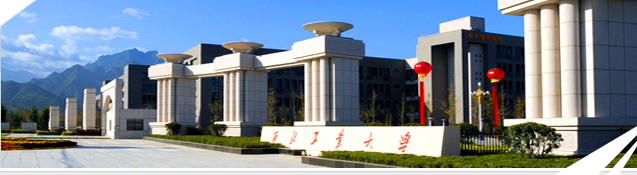
\includegraphics[width = 0.9\textwidth]{npu}
\FigureBiCaption{西北工业大学长安校区}{}
\label{fig:intro-npu}
\end{figure}

\BiSection{其他说明}{ }

论文使用pdflatex编译,在Linux系统下如果需要使用Windows下的字体,可能需
需要制作字体,具体方法请上网Google。另外,也可尝试对字体支持更好的
xetex编译,但可能需要进行一些修改。

main.tex中有每一章从右侧/奇数页开始的选项(openleft),但插入的并不是一
个完全的空白页。如需空白页,可以关闭openleft选项,然后手动在合适位置使
用如下命令插入空白页:
\begin{verbatim}
\newpage
~~~\vspace{1em}
\thispagestyle{empty}
\end{verbatim}

编译时直接使用\texttt{make}命令,得到\texttt{main\_pdflatex.pdf}文件。

